\section{Multi data inference}
One promising path is the use of multiple type of data to train and infer. For example, one could use \gls{lidar} surveys combined with spatial photography to produce stronger and more robust model. In our case, we are lucky enough to have vast swath of terrain already surveyed by \gls{lidar}, and high resolution geospatial photography is fairly easy to obtain. Combining those two types of data could help the network become more robust as it would have access to more information. %TODO:reformulate

Combining those two type of data might require the use of a modified file format, able to use 4 channels: 1 for the \gls{lidar} grayscale survey, and 3 for the RGB values of the satellite photography. Modifications to the detection network might also have to be done to be able to use such a file format. 
\section{Semantic Segmentation}%TODO: find paper

\begin{figure}[H]
  \centering
  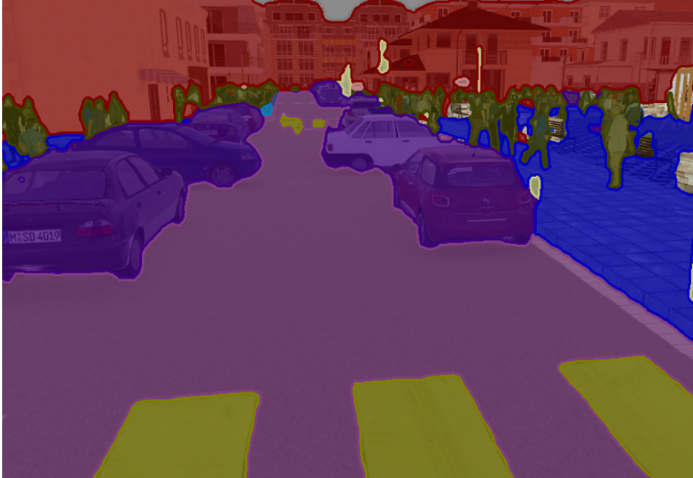
\includegraphics[width=0.7\textwidth]{semantic-segmentation.png}
	\caption[]{Example of semantic segmentation on a street scene.}
  \label{fig:semSeg}
\end{figure}

Segmentation of object at the pixel level, instead of using bounding boxes could be done. While bounding boxes are enough for precise location of objects, it might not be enough to compute some attributes of those objects, like their size or orientation. Bounding boxes also poses an issue with objects that are not aligned in the same way. While some techniques allows for rotation of bounding boxes, such as this paper by Lou, Pan and Lei\cite{louPanLei2017}, more precise segmentation could be a useful and interesting study path. 

State of the Art models uses fully convolutional networks or U-Nets. Mask-RCNN\cite{maskrcnn} is one of the most well known model capable of semantic segmentation, but since then many newer and more performant networks have been published such as Deep Lab\cite{deepLab}, Fast-FCN\cite{fastFCN} or Gated-SCNN\cite{gated-scnn}. A more comprehensive review of the state of the art should obviously be done, and modifications to those models might be necessary to achieve good results on the particular type of data generated by Archaeological Remote Sensing.
